% 页面设置
\documentclass[12pt, a4paper]{article} % 字号:12,纸张:A4
\usepackage[top=2.54cm, bottom=2.54cm, left=3.18cm,right=3.18cm]{geometry} % 页边距设置
% 字体设置
\usepackage[UTF8]{ctex}
\usepackage{fontspec} % 设置字体
%\setCJKmainfont{SimSun}[AutoFakeBold=true, BoldFont={SimHei}, ItalicFont={KaiTi}] % 正文字体
%\setCJKsansfont[AutoFakeBold=3]{KaiTi} % 无衬线字体
%\setCJKmonofont[AutoFakeBold=3]{SimHei} % 等宽字体
\setmainfont{Times New Roman} % 设置主字体为新罗马体
% 文本设置
\usepackage{enumerate} % 支持小标题编号
\linespread{1.5} % 行间距1.5倍
\usepackage{indentfirst}%首段缩进
\setlength{\parindent}{2em} % 首行缩进两字符
\usepackage[hidelinks]{hyperref} % 目录添加超链接
\usepackage{zhnumber} % 章节标题中文显示
\usepackage[cmyk]{xcolor} % 文字彩色显示
% 数学支持
\usepackage{amsmath} % 数学公式支持
\usepackage{amssymb} % 数学符号支持
\usepackage{bm} % 公式加粗
\usepackage{mathrsfs} % 花体字母
\usepackage{yhmath} % 更多的数学符号
% 图片设置
\usepackage{caption} % 插入图片标题
\usepackage{float} % 控制图片位置
\usepackage{subfigure} % 图片并排
\usepackage{booktabs} % 插入表格
% 表格设置
\usepackage{multirow} % 表格自动换行
\usepackage{bigstrut} % 表格间距
\usepackage{rotating} % 表格旋转
\usepackage{tabularx} % 表格宽度
\usepackage{colortbl} % 表格颜色
\usepackage{graphicx} % 表格自动宽度

\title{第二章 \ \ \ 模型评估与选择} % 文章标题
\author{Castor Ye} % 文章作者
\date{} % 文章时间

\begin{document} % 文档从这里开始。
\maketitle % 按照预定的模板把上面那些信息排好。
\newtheorem{definition}{定义}[section]
\newtheorem{theorem}{定理}[section]
\newtheorem{example}{例}[section]
\newtheorem{solution}{题解}
\newtheorem{algorithm}{算法}
\newtheorem{axiom}{公理}
\newtheorem{property}{性质}
\newtheorem{proposition}{命题}
\newtheorem{lemma}{引理}
\newtheorem{corollary}{推论}[section]
\newtheorem{remark}{注解}
\newtheorem{condition}{条件}
\newtheorem{conclusion}{结论}
\newtheorem{assumption}{假设}
\renewcommand{\figurename}{图} % 将图片序号改为图
\renewcommand{\tablename}{表} % 将表格序号改为表
%%%%%%%%%%%%%%%%%%%%%%%%%%%%%%%%%%%%%%%%%%%%%%%%%%%%%%%%%%%%%%%%%%%%%%%
% 文章内容从此开始
\section{经验误差与过拟合}

一般地,我们把学习器的实际预测输出与样本的真实输出之间的差异称为“误差”(error),学习器在训练集上的误差称为“训练误差”(training error)或“经验误差”(empirical error),在新样本上的误差称为“泛化误差”(generalization error)。

显然,我们希望得到的是在新样本上表现很好地学习器,即泛化误差小的学习器。因此我们应该从训练样本中尽可能学出适用于所有潜在样本的“普遍规律”。然而,当学习器把训练集学得“太好”的时候,即把一些训练样本的自身特点当成了普遍特征,这种情况在机器学习中称为“过拟合”(overfitting)。同时也有学习能力不足的时候,即训练集的基本特征都没有学习出来,我们称之为“欠拟合”(underfitting)。

可以得知:在过拟合问题中,训练误差十分小,但测试误差较大;在欠拟合问题中,训练误差和测试误差都比较大。目前,欠拟合问题比较容易克服,例如增加迭代次数等。但过拟合问题还没有十分好的解决方案,过拟合是机器学习面临的关键障碍。

\section{评估方法}

在现实任务重,我们往往有多种算法可供选择,那么我们应该选择哪一个算法才是最合适的呢?如上所述,我们希望得到的是泛化误差小的学习器,理想的解决方案是对模型的泛化误差进行评估,然后选择泛化误差最小的那个学习器。但是,泛化误差指的是模型在所有新样本上的适用能力,我们无法直接获得泛化误差。

因此,通常我们采用一个“测试集”来测试学习器对新样本的判别能力,然后以“测试集”上的“测试误差”作为“泛化误差”的近似。显然,我们选择的测试集应与训练集互斥。

可是,我们只有一个包含 $m$ 个样例的数据集 $D = \{(x_1, y_1), (x_2, y_2), \cdots, (x_m, y_m)\}$,既要训练,又要测试,怎么才能做到呢?我们可以通过对 $D$ 进行适当的处理,从中生成训练集 $S$ 和测试集 $T$,下面介绍几种常见的做法:

\subsection{留出法}

“留出法”(hold-out)直接将数据集 $D$ 划分为两个互斥的集合,其中一个集合作为训练集 $S$,另一个作为测试集 $T$,即 $D = S \cup T, S \cap T = \emptyset$。在 $S$ 上训练模型后,用 $T$ 来评估其测试误差,作为对泛化误差的估计。

由于划分的随机性,单词的留出法结果往往不够稳定,一般要采用若干次随机划分,重复实验取平均值的做法。

\subsection{交叉验证法}

“交叉验证法”(cross validation)先将数据集 $D$ 划分为 $k$ 个大小相似的互斥子集,即 $D = D_1 \cup D_2 \cdots \cup D_k, D_i \cap D_j = \emptyset$。每个自己 $D_i$ 都尽量保持数据分布的一致性,即从 $D$ 中通过分层采样得到。

交叉验证法的思想是:每次用 $k - 1$ 个子集的并集作为训练集,余下的那个子集作为测试集;这样就可以获得 $k$ 组不同训练集和测试集,即进行 $k$ 次训练和测试,最终返回 $k$ 次测试结果的均值。

交叉验证法也称“$k$ 折交叉验证”,$k$ 最常用的取值为 $10$,下图给出了 $10$ 折交叉验证的示意图:

\begin{figure}[H]
    \centering
    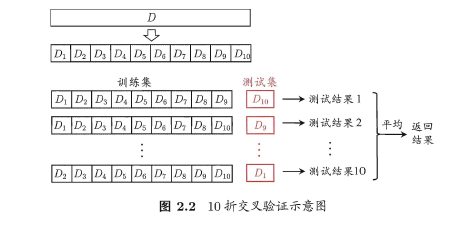
\includegraphics[width=0.7\textwidth]{../img/2-1-10折交叉验证.png}
    \caption{10 折交叉验证}
    \label{fig:10 折交叉验证}
\end{figure}

与留出法类似,将数据集 $D$ 划分为 $k$ 个子集的过程具有随机性,因此 $k$ 折交叉验证通常也要重复 $p$ 次,称为 $p$ 次 $k$ 折交叉验证。常见的是 $10$ 次 $10$ 折交叉验证。

\subsection{自助法}

我们希望评估的是用 $D$ 训练出的模型,但在留出法和交叉验证法中,由于保留了一部分样本用于测试,因此实际评估的模型所使用的训练集比 $D$ 小,这必然会引入一些因训练样本规模不同而导致的估计偏差。

“自助法”(bootstrapping)的基本思想是:给定包含 $m$ 个样本的数据集 $D$,我们对它进行采样产生数据集 $D ^\prime$,每次随机从 $D$ 中挑选一个样本,将其拷贝放入 $D ^\prime$,然后再将该样本放回初始数据集 $D$ 中,使得该样本在下次采样时仍有可能被采到。重复执行 $m$ 次,我们就得到了一个包含 $m$ 个样本的数据集 $D ^\prime$。可以得知,在 $m$ 次采样中始终不被采到的概率是:

\begin{equation}
    \lim_{m \to \infty} (1 - \frac{1}{m})^m = \frac{1}{e} \approx 0.368
\end{equation}

这样,通过自助采样,初始样本集 $D$ 中大约有 $36.8\%$ 的样本未出现在采样数据集 $D ^\prime$ 中。于是,我们可以将 $D ^\prime$ 作为训练集,$D - D^\prime$ 作为测试集。

自助法在数据集较小,难以有效划分训练集和测试集时很有用,但由于自助法产生的数据集(随机抽样)改变了初始数据集的分布,因此引入了估计偏差。在数据集足够时,留出法和交叉验证更加常用。

\subsection{调参与最终模型}

大多数学习算法都有些参数(parameter)需要设定,参数配置不同,学得模型的性能往往有显著区别。因此,在进行模型评估与选择时,除了要对适用的学习算法的选择,还需对算法参数进行设定,这就是通常所说的“参数调节”或简称“调参”(parameter tuning)。


\end{document}